\documentclass{docs}

%--- 基本パッケージ ---%
\usepackage{makecell} % 表のセルの配置
\usepackage{pgfgantt} % ガントチャート作成
\usepackage{tabularx} % 表の幅を調整
\usepackage{here} % 図や表の位置を固定 (H)

%--- 文書情報 ---%
\title{システム提案書}
\renewcommand\theadfont\bfseries

\begin{document}

%%%%%%%%%%%%%%%%%%%%%%%%%%%%%%%%%%%%%%%%%%%%%%%%%%%%%%%%%%%%
% 1. 現状の課題
%%%%%%%%%%%%%%%%%%%%%%%%%%%%%%%%%%%%%%%%%%%%%%%%%%%%%%%%%%%%
\section{現状の課題}\label{sec:issues}
%--- システム開発に至った背景や、解決したい社会課題の概要を記述。---%
2024年に高知県を訪れた県外観光客入込数は、対前年比94.3\,\%、約268,000人減の
4,453,000人と推計され、過去最高である前年に比べて減少とはなりましたが、
過去2番目となりました。
また、観光施設の利用状況において、利用者数が最も
多かったのは「高知県立牧野植物園」で314,883人でした\cite{kochi_tourism_stat}。
これらのことから、前年に放映された連続テレビ小説「らんまん」が
観光客の動向に大きく影響を与えていると考えられます。

このように、映像作品やコンテンツは観光誘致において、重要な役割を果たしています。

しかし、上記データが示す「らんまん」効果の反動減は、
コンテンツツーリズムが抱える最大の問題、すなわち
「ブームの一過性」と「観光の持続可能性の欠如」を
象徴しています。内閣官房の資料\cite{sangiin2012}でも、放送終了後に
ブームが沈静化する課題が指摘されています。
高知県自身も、この反動減を課題として認識しており、
次の「あんぱん」放送に向け「誘客の拡大と県内周遊の強化を図る」
ことを最重要課題の一つとして掲げています\cite{kochi_r7_plan}。

本システムは、聖地巡礼という観光体験を最大化し、観光客と地域事業者を繋ぐことで、
この課題の解決を目指すものです。
以下に、高知県の公式な課題認識\cite{kochi_dx_plan}を踏まえた、
各ステークホルダーの視点での課題を列挙します。
\subsection{行政の視点}
%--- 行政が抱える課題を箇条書きで記述。---%
\begin{itemize}
\item \emph{観光の一極集中と周遊の不足:}
	「らんまん」ブームが牧野植物園という特定の施設に集中したように、
	観光客が特定の有名な聖地(点)のみを訪れるだけで、県内の他地域への周遊(面)に進みません。
	これは観光庁が対策を進めるオーバーツーリズム(観光公害)の一形態\cite{kanko_overtourism}であり、
	「特定の場所への観光客の過度な集中」は、交通渋滞や混雑による
	住民生活への負担、および観光客自身の満足度低下を招きます。
	さらに、「仁淀ブルー」で知られるにこ淵の事例\cite{nikobuchi_mlit}では、
	にこ淵を見て帰るだけの日帰り客が多く、地域での周遊や宿泊が見られないため
	地域にお金は落ちない、という経済的な課題も明確に指摘されています。

	\item \emph{観光データの不足と活用の遅れ:}
	高知県が公式に発表した「高知県デジタル化推進計画」\cite{kochi_dx_plan}において、
	最重要課題の一つとして「データを活用した効果的なプロモーションや
	観光客のニーズに即したコンテンツ造成…が十分でない」ことが明記されています。
	これは、行政が観光客の行動データを強く求めている明確な根拠です。
	現状では、聖地巡礼客が「どこから来て」「どこを周り」「どこで消費せず離脱しているか」
	という詳細なデータが不足しており、効果的な周遊施策の立案が困難となっています。

	\item \emph{観光の持続の困難さ:}
	前述の通り、コンテンツの放送・公開終了後、
	急激に観光客が減少する反動減が公式に確認されています\cite{kochi_r7_plan}。
	内閣官房の資料\cite{cas_kadokawa}でも、ブームを一過性に終わらせず、
	持続的な稼ぐ力に繋げることが国のコンテンツ政策の課題として挙げられています。
\end{itemize}

\subsection{消費者の視点}
%--- 消費者が抱える課題を箇条書きで記述します。---%
\begin{itemize}
	\item \emph{周辺情報の不足と分かりづらさ:}
	最も深刻な課題は、行政の課題\cite{kochi_dx_plan}と表裏一体です。
	高知県デジタル化推進計画\cite{kochi_dx_plan}は、
	観光客の周遊・滞在促進につながる情報発信・コンテンツが不足
	していることを県の課題として明確に認めています。
	また、情報発信の方法にも問題があると
	考えられます。JTB総合研究所の調査\cite{jtb_trc_2017}では
	「県や町単位のため、近隣でどのような観光ができるのかわかりにくい」という不満が
	多いとされており、
	周遊の機会が失われていると考えられます。

	\item \emph{情報の散在と信頼性の欠如:}
	聖地巡礼の情報は、ファンがSNSやWeb検索に頼らざるを得ない状況にあります。
	しかし、高知県の観光情報に関するアンケート調査では、
	公式情報に対してすら「サイトの更新情報が古い」
	「タイムリーな情報が少ない」といった信頼性への不満が指摘されています\cite{kochi_tech_2017}。

	\item \emph{現地での体験価値の低さ(没入感の不足):}
	TOPPAN株式会社が記したコラム\cite{toppan2025}によれば、聖地巡礼の醍醐味は
	「作品の世界観を深く味わうこと」、すなわち「没入感」
	($={}$作品世界との一体感を味わう体験)にあるとされています。
	ファンは、作中と「同じ角度で写真を撮る」「同じ雰囲気を感じる」
	といった、より深い体験を求めていますが、現地では風景を見るだけで
	その具体的な方法が分からず、没入感が阻害されています。
\end{itemize}


\subsection{事業者の視点}
%--- 事業者が抱える課題を箇条書きで記述.---%
\begin{itemize}
\item \emph{集客機会の損失:}
	にこ淵の事例\cite{nikobuchi_mlit}のように、聖地巡礼者が
	その観光スポットのみに集中するのみで入店に繋がらず、収益が得られないといったことがあります。
	これは、高知県の観光課題としてマーケティング不足が指摘される通り\cite{kochi_tech_2017}、
	個々の事業者がニッチなファン層へ効果的に
	アプローチする手段を持っていないからです。

	\item \emph{情報発信の難しさ:}
	作品のファン(特定の興味を持つ層)に対して、
	自店の魅力を発信する適切なプラットフォームが存在しません。

	\item \emph{コラボレーション(広告)の障壁:}
	野村総合研究所のコンサルタントの指摘\cite{nri2024}の通り、
	コンテンツの版権(ライセンス)契約の調整は、
	事業者にとって最も大きな課題です。
	個店が低コストでファン向けの商品開発や
	コラボ広告を行うことは事実上不可能です。
\end{itemize}

%%%%%%%%%%%%%%%%%%%%%%%%%%%%%%%%%%%%%%%%%%%%%%%%%%%%%%%%%%%%
% 2. 課題解決のための提案
%%%%%%%%%%%%%%%%%%%%%%%%%%%%%%%%%%%%%%%%%%%%%%%%%%%%%%%%%%%%
%--- 上記の課題をどのように解決するのか、システムのコンセプトを記述
\section{課題解決のための提案}
上記の課題、特に高知県が公式に特定した「データ活用の不足」と「周遊コンテンツの不足」\cite{kochi_dx_plan}
を解決するため、AIとUGC(ユーザー生成コンテンツ)を活用した
対話型の聖地巡礼サポートシステム「SceneTrip」を提案します。
本システムは、特定のIPに依存せず、ファンが主体となって情報を
創り上げるプラットフォームとして機能し、持続可能な観光エコシステムの
構築を目指します。

\subsection{解決策1: AIによる対話型コンシェルジュ機能}
利用者の周辺情報の不足という課題に対し、AIチャットボットが
「聖地巡礼に詳しい旅の相談相手」として対話形式で応えます。
\begin{itemize}
	\item \emph{パーソナライズされた巡礼プランの提案:}
	高知県デジタル化推進計画\cite{kochi_dx_plan}が課題とする
	周遊・滞在促進につながる情報を、AIが利用者の興味や時間に応じて
	最適化して提供します。
	\item \emph{自然言語による情報検索:}
	「この近くにある、作中に出てきたような風景や景色が眺められる喫茶店は?」
	といった曖昧な質問に対しても、AIが口コミやタグ情報を解析して
	最適な場所を推薦します。
\end{itemize}

\subsection{解決策2: UGCと「お楽しみ機能」による周遊促進と体験価値向上}
行政の周遊促進と一極集中対策、および利用者の体験価値の課題に対し、
UGCとゲーム的な要素を組み合わせます。
\begin{itemize}
	\item \emph{実績バッジ(スタンプラリー機能):}
	各聖地や協力店舗へのチェックイン、写真投稿といった活動に応じて
	ポイントを付与します。特定のクエスト(例: 聖地から1\,km以内の飲食店訪問)を
	クリアさせ、観光客を能動的に分散・周遊させます。
	\item \emph{フォトスポット投稿・共有機能:}
	利用者の没入感の課題を解決します。ユーザーが「作中のあのシーンの
	ように撮れる」具体的な場所や角度を写真付きで投稿・共有します。
	これにより、他のユーザーはその情報を元に、より没入感の高い写真撮影体験ができます。
\end{itemize}

\subsection{解決策3: 地域事業者との連携プラットフォームとデータ分析}
事業者および行政の課題に対し、情報発信とデータ活用の仕組みを提供します。
\begin{itemize}
	\item \emph{事業者向け情報発信ツール:}
	\begin{itemize}
		\item \emph{Googleマップ等との優位性:}
		Googleマップが不特定多数に向けた汎用的な情報掲載であるのに対し、
		本システムは「聖地巡礼」という明確な目的意識を持つファン層に
		限定して直接アプローチできます。
		\item ライセンス契約\cite{nri2024}の障壁なしに、地域の店舗がアプリ内に
		クーポンや、「巡礼者歓迎!」「作中の○○に似たメニューがあります」といった
		ファン向けの特別な商品・サービス情報を簡単に掲載できる機能を提供します。
	\end{itemize}
	\item \emph{データ駆動型観光の実現:}
	\begin{itemize}
		\item \emph{高知県デジタル化推進計画\cite{kochi_dx_plan}}が
		最重要課題とするデータ活用を本システムが担います。
		\item \emph{収集方法:}
		利用者の許諾を得た上で、アプリのチェックイン情報や、
		クーポンの利用履歴、AIへの検索クエリ、閲覧された口コミ、写真を収集します。
		\item \emph{分析・提供方法:}
		個人を特定しない形でデータを統計処理し、「訪問者の周遊パターン」
		「人気のフォトスポット」「時間帯別混雑ヒートマップ」
		「クーポン利用率」等を可視化し、行政や登録事業者向けに
		専用の分析ページ(ダッシュボード)を提供します。
	\end{itemize}
\end{itemize}

%%%%%%%%%%%%%%%%%%%%%%%%%%%%%%%%%%%%%%%%%%%%%%%%%%%%%%%%%%%%
% 3. 機能概要・前提条件・制約事項
%%%%%%%%%%%%%%%%%%%%%%%%%%%%%%%%%%%%%%%%%%%%%%%%%%%%%%%%%%%%
\subsection{機能概要}
\subsubsection{利用者向け機能}
\begin{itemize}
	\item \emph{AIによる旅の相談機能(対話型)}
	\begin{itemize}
		\item 観光地・施設検索
		\item 経路検索
		\item \emph{外部マップアプリ連携機能}
		(検索した目的地をGoogleマップ等に自動入力します)
	\end{itemize}
	\item \emph{UGC(口コミ・写真)機能}
	\begin{itemize}
		\item 口コミ・評価
		\item フォトスポット投稿・共有
	\end{itemize}
	\item \emph{お楽しみ機能(スタンプラリー)}
	\begin{itemize}
		\item チェックイン機能
		\item 実績バッジ
	\end{itemize}
	\item クーポンの受け取り
\end{itemize}

\subsubsection{事業者・行政向け機能}
\begin{itemize}
	\item 広告掲載
	\item \emph{観光データの分析・提供(専用ページ)}
	\item \emph{データ連携機能(API)}
	(※高度な分析をする専門組織向け)
	\item クーポンの発行
\end{itemize}

\subsection{前提条件}
%--- システムが動作するための前提条件を箇条書きで記述。---%
\begin{itemize}
	\item 利用者がインターネット接続可能なPCまたはスマートフォンを
	所有していること。
	\item 利用者が本システムの利用規約に同意していること。
	\item 一部の機能は会員登録が必須であること。
\end{itemize}

\subsection{制約事項}
%--- システム開発や運用における制約事項を箇条書きで記述。---%
\begin{itemize}
	\item 個人情報保護法を遵守し、情報漏洩を防ぐ仕様であること。
	\item システム管理者による不適切な投稿の監視・削除が可能であること。
\end{itemize}

%%%%%%%%%%%%%%%%%%%%%%%%%%%%%%%%%%%%%%%%%%%%%%%%%%%%%%%%%%%%
% 4. 情報・金銭の流れ
%%%%%%%%%%%%%%%%%%%%%%%%%%%%%%%%%%%%%%%%%%%%%%%%%%%%%%%%%%%%
\section{情報・金銭の流れ}
\subsection{情報の流れ}
%--- システムにおける情報の流れを図で示す。---%
\begin{figure}[H]
	\centering
	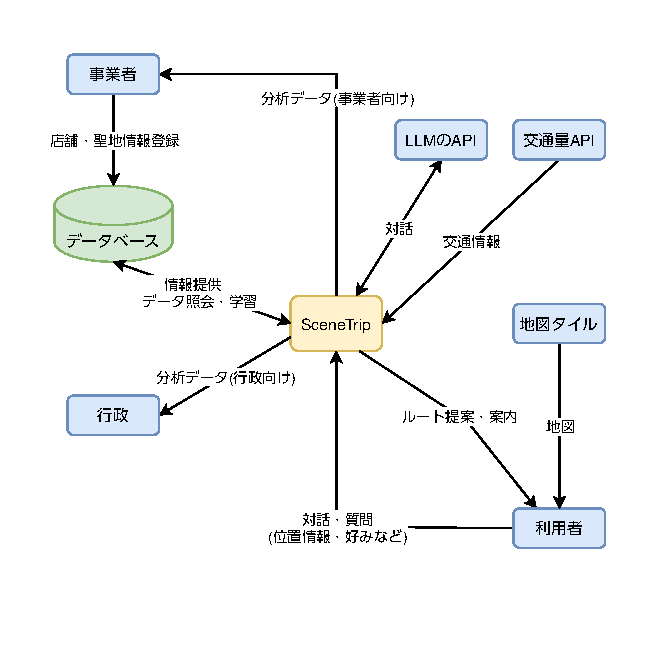
\includegraphics[bb=24.047999 46.835999 290.862765 284.219991,clip,scale=.8]{softinfo.pdf}
	\caption{SceneTripにおける情報の流れ}\label{fig:info}
\end{figure}

\subsection{金銭の流れ}
%--- システムにおける金銭(またはポイント)の流れを図で示す---%
\begin{figure}[H]
	\centering
	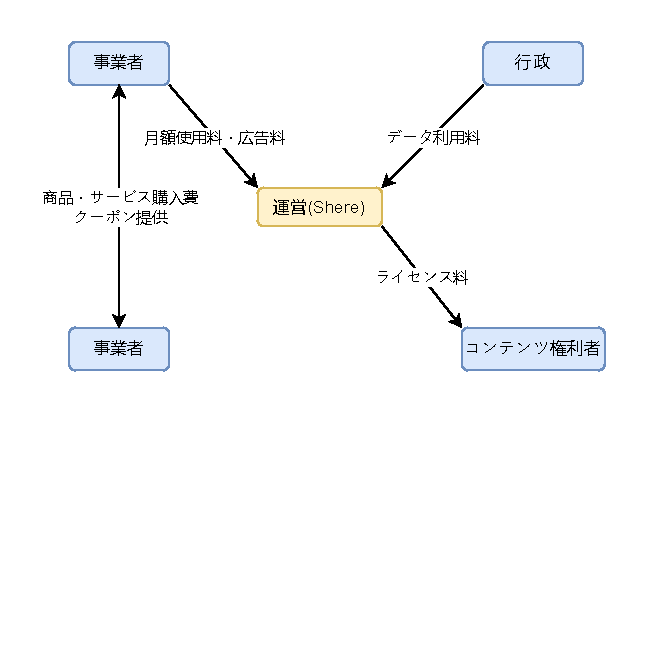
\includegraphics[bb=39.735702 77.129998 539.783984 98.063997,clip,scale=.8]{softmoney.pdf}
	\caption{SceneTripにおける金銭の流れ}\label{fig:money}
\end{figure}


%%%%%%%%%%%%%%%%%%%%%%%%%%%%%%%%%%%%%%%%%%%%%%%%%%%%%%%%%%%%
% 5. 想定する利用者
%%%%%%%%%%%%%%%%%%%%%%%%%%%%%%%%%%%%%%%%%%%%%%%%%%%%%%%%%%%%
\section{想定する利用者}
%--- このシステムの主なターゲットユーザーを箇条書きで記述。---%
\begin{itemize}
	\item 聖地巡礼者
	\item 周遊・体験を重視するアクティブな観光客
	\item デジタルネイティブな情報収集者
\end{itemize}

%%%%%%%%%%%%%%%%%%%%%%%%%%%%%%%%%%%%%%%%%%%%%%%%%%%%%%%%%%%%
% 6. ハードウェア構成・ソフトウェア構成
%%%%%%%%%%%%%%%%%%%%%%%%%%%%%%%%%%%%%%%%%%%%%%%%%%%%%%%%%%%%
\section{ハードウェア構成・ソフトウェア構成}
\subsection{ハードウェア構成}
%--- システムに必要なハードウェア構成を表で示す。---%
\begin{table}[H]
	\centering
	\caption{ハードウェア構成}\label{tab:hardware}
	\begin{tabularx}{0.9\textwidth}{|l|p{9\zw}|X|p{10\zw}|}
		\hline
		\thead{項目} & \thead{種類} & \thead{数量} & \thead{備考} \\ \hline
		メインサーバ & OCI Compute & 1台 & Always Freeサービス(無料枠)\\ \hline
		データベースサーバ & OCI Compute & 1台 & Always Freeサービス(無料枠)\\ \hline
		管理者端末 & PCおよびスマートフォン & 管理者数 & \\ \hline
		利用者端末 & PCおよびスマートフォン & 利用者数 & \\ \hline
	\end{tabularx}
\end{table}

\subsection{ソフトウェア構成}
%--- システムに必要なソフトウェア構成を表で示す。---%
\begin{table}[H]
	\centering
	\caption{ソフトウェア構成}\label{tab:software}
	\begin{tabularx}{0.9\textwidth}{|l|X|l|}
		\hline
		\thead{項目} & \thead{ソフトウェア} & \thead{備考} \\ \hline
		Webサーバ & Nginx & \\ \hline
		データベース & MariaDB & \\ \hline
		バックエンド & PHP(Laravel) & \\ \hline
		フロントエンド & TypeScript & \\ \hline
		端末OS & Android、Linux、Windows、iOS、macOS & \\ \hline
		端末ブラウザ & Firefox、Google Chrome、Safari & \\ \hline
		LLM & Gemini 2.5 Flash-Lite & Google AI Studioを使用 \\ \hline
		地図 & OpenStreetMap & \\ \hline
		交通情報 & 国土交通省交通量API & \\ \hline
	\end{tabularx}
\end{table}

%%%%%%%%%%%%%%%%%%%%%%%%%%%%%%%%%%%%%%%%%%%%%%%%%%%%%%%%%%%%
% 7. 運用・保守
%%%%%%%%%%%%%%%%%%%%%%%%%%%%%%%%%%%%%%%%%%%%%%%%%%%%%%%%%%%%
\section{運用・保守}
\subsection{運用}
%--- システムリリース後の日常的な運用業務を箇条書きで記述。---%
\begin{itemize}
	\item システムの稼働監視
	\item 定期的なデータバックアップ
	% \item 口コミ審査
	\item 口コミへの不適切な投稿の監視
	\item セキュリティ監視
	\item 事業者データの登録・管理
	\item 行政への分析データ提供
	\item 問い合わせ対応
\end{itemize}

\subsection{保守}
%--- システムを正常に維持するための保守業務を箇条書きで記述。---%
\begin{itemize}
	\item インフラのメンテナンス
	\item 障害発生時の原因究明と復旧作業
	\item バグや不具合の修正
	\item OSやミドルウェアのアップデート
\end{itemize}

%%%%%%%%%%%%%%%%%%%%%%%%%%%%%%%%%%%%%%%%%%%%%%%%%%%%%%%%%%%%
% 8. 費用対効果
%%%%%%%%%%%%%%%%%%%%%%%%%%%%%%%%%%%%%%%%%%%%%%%%%%%%%%%%%%%%
\section{費用対効果}
\subsection{効果}
%--- システム導入によって得られる定性的な効果を記述。---%
システムの導入により、\cref{sec:issues}に挙げた
各ステークホルダーの視点での課題が解決すると考えられます。

\subsection{収益}
%--- 5年間など、特定の期間における収益モデルと予測金額を記述。---%
収益は、事業者からの月額利用料、広告収入、行政からの手数料を想定します。
\begin{itemize}
	\item \emph{事業者利用料:} $\text{3,000円/月}\times\text{300事業者}
	\times\text{60ヶ月}=\text{54,000,000円}$
	\item \emph{広告収入:} $\text{100,000円/月}\times\text{60ヶ月}
	=\text{6,000,000円}$
	\item \emph{データ利用手数料:} $\text{50,000円/月}\times\text{60ヶ月}
	=\text{3,000,000円}$
\end{itemize}
\emph{5年間の総収益: 63,000,000円}

\subsection{費用}
%--- 開発にかかる初期費用と、運用にかかる費用を表や数式で示します。---%
\begin{itemize}
	\item \emph{初期費用(開発費):}
		\begin{itemize}
			\item 人件費: $\text{10,000,000円/年}\times\text{7名}\times\text{5ヶ月}
			\sim\text{29,166,667円}$
			\item その他(機材費など): 0円\\
			(開発に関わる環境や機材の費用は人件費に含む)
		\end{itemize}
		\emph{初期費用合計: 29,166,667円}
	\item \emph{運用費用(5年間):}
		\begin{itemize}
			\item サーバ費用: $\text{0円/月}\times\text{60ヶ月}
			=\text{0円}$
			\item 維持管理費(人件費など): $\text{2,916,667円/年}\times\text{60ヶ月}
			\sim\text{14,583,333円}$\\
			(年間費用は初期費用の1割として計算)
		\end{itemize}
		\emph{5年間の運用費用合計: 14,583,333円}
\end{itemize}
\emph{5年間の総費用: 43,750,000円}

\subsection{利益}
%--- 5年間など、特定の期間における利益を計算。---%
5年間で得られる利益は以下の通りです。
\begin{gather*}
	\text{総収益} - \text{総費用} = \text{利益}\\
	\text{63,000,000円} - \text{43,750,000円} = \text{19,250,000円}
\end{gather*}

%%%%%%%%%%%%%%%%%%%%%%%%%%%%%%%%%%%%%%%%%%%%%%%%%%%%%%%%%%%%
% 9. 開発体制と工程計画
%%%%%%%%%%%%%%%%%%%%%%%%%%%%%%%%%%%%%%%%%%%%%%%%%%%%%%%%%%%%
\section{開発体制と工程計画}

%--- 開発チームの体制について記述. ---%
本システムの開発は、高知工科大学情報学群の学生7名からなるグループShareが
行います。

%--- 開発スケジュール(ガントチャートなど)を図で示す。---%
また、開発モデルとしてウォーターフォールモデルを採用し、
\cref{fig:gantt}に示す工程で開発します。
\begin{figure}[H]
	\centering
	\begin{ganttchart}[
		canvas/.append style={fill=none,ultra thick},
		title/.append style={fill=none},
		title height=1,
		title label text={\emph{#1}},
		hgrid={draw},
		x unit=16pt,
		y unit chart=34pt,
		bar/.style={},
		bar label node/.append style={align=right},
		left label/.style={
			bar/.style={draw,thick,fill=gray!60},
			bar inline label anchor=west,
			bar inline label node/.style={anchor=east},
			inline,
		},
		right label/.style={
			bar inline label anchor=east,
			bar inline label node/.style={anchor=west},
			inline,
		},
	]{0}{20}
		\gantttitle{2025年}{14}
		\gantttitle{2026年}{7}\\
		\gantttitle{9月}{2}
		\gantttitle{10月}{4}
		\gantttitle{11月}{4}
		\gantttitle{12月}{4}
		\gantttitle{1月}{4}
		\gantttitle{2月}{3}\\
		\ganttbar{要求分析}{0}{0}
		\ganttbar[left label]{10/2}{2}{5}
		\ganttbar[right label]{10/30}{2}{5}\\
		\ganttbar{外部設計}{0}{0}
		\ganttbar[left label]{10/30}{6}{9}
		\ganttbar[right label]{12/1}{6}{9}\\
		\ganttbar{内部設計}{0}{0}
		\ganttbar[left label]{12/1}{10}{12}
		\ganttbar[right label]{12/22}{10}{12}\\
		\ganttbar{コーディング\&\\単体テスト}{0}{0}
		\ganttbar[left label]{12/22}{13}{15}
		\ganttbar[right label]{1/15}{13}{15}\\
		\ganttbar{結合・総合テスト}{0}{0}
		\ganttbar[left label]{1/15}{16}{16}
		\ganttbar[right label]{1/22}{16}{16}\\
		\ganttbar{βテスト}{0}{0}
		\ganttbar[left label]{1/22}{17}{18}
		\ganttbar[right label]{2/5}{17}{18}
	\end{ganttchart}
	\caption{工程計画}\label{fig:gantt}
\end{figure}

%%%%%%%%%%%%%%%%%%%%%%%%%%%%%%%%%%%%%%%%%%%%%%%%%%%%%%%%%%%%
% 参考文献
%%%%%%%%%%%%%%%%%%%%%%%%%%%%%%%%%%%%%%%%%%%%%%%%%%%%%%%%%%%%
\begin{thebibliography}{99}
	%--- 提案書作成にあたり参考にした文献やWebサイトを記述。---%
	\bibitem{kochi_tourism_stat}
	高知県,
	“県外観光客入込・動態調査について | 高知県”,
	2025年,
	\url{https://www.pref.kochi.lg.jp/doc/2017090600162/},
	2025年10月20日閲覧.

	\bibitem{sangiin2012}
	筒井隆志
	“コンテンツツーリズムの新たな方向性 ~地域活性化の手法として~”,
	2013年,
	\url{https://www.sangiin.go.jp/japanese/annai/chousa/keizai_prism/backnumber/h25pdf/201311002.pdf},
	2025年10月28閲覧.

	\bibitem{kochi_r7_plan}
	高知県,
	“令和7年度の取り組みの強化のポイント 【観光分野】”,
	2025年,
	\url{https://www.pref.kochi.lg.jp/doc/2024121100065/file_contents/file_2025231165656_1.pdf},
	2025年10月23日閲覧.

	\bibitem{kochi_dx_plan}
	高知県,
	“第2期高知県デジタル化推進計画(令和6年度版)”,
	2024年,
	\url{https://www.pref.kochi.lg.jp/doc/2024032700101/file_contents/file_20243284151622_1.pdf},
	2025年10月24日閲覧.

	\bibitem{kanko_overtourism}
	国土交通省観光庁,
	“オーバーツーリズムの未然防止・抑制に向けた取組 | 持続可能な観光地域づくりのための体制整備等の推進 | 持続可能な観光地域づくり戦略 | 観光政策・制度 | 観光庁”,
	2025年,
	\url{https://www.mlit.go.jp/kankocho/seisaku_seido/kihonkeikaku/jizoku_kankochi/jizokukano_taisei/overtourism.html},
	2025年10月24日閲覧.

	\bibitem{nikobuchi_mlit}
	国土交通省観光庁,
	“にこ淵を中心とした仁淀川流域のオーバーツーリズム対策”,
	2025年,
	\url{https://www.mlit.go.jp/kankocho/content/001878840.pdf},
	2025年10月23日閲覧.

	\bibitem{cas_kadokawa}
	内閣官房 新しい資本主義実現本部事務局・内閣府 知的財産戦略推進事務局,
	“基礎資料(第26回新しい資本主義実現会議の基礎資料の改訂・再編版)”,
	2024年,
	\url{https://www.cas.go.jp/jp/seisaku/atarashii_sihonsyugi/wgkaisai/contents_dai1/siryou3.pdf},
	2025年10月24日閲覧.

	\bibitem{jtb_trc_2017}
	JTB総合研究所,
	“スマートフォンの利用と旅行消費に関する調査(2017)”,
	2017年,
	\url{https://www.tourism.jp/wp/wp-content/uploads/2017/12/smartphone-2017.pdf},
	2025年10月27日閲覧.

	\bibitem{kochi_tech_2017}
	中司絵里花,
	“高知県の観光課題の構造分析”,
	2018年,
	\url{https://www.kochi-tech.ac.jp/library/ron/pdf/2017/03/14/a1180459.pdf},
	2025年10月23日閲覧.

	\bibitem{toppan2025}
	TOPPAN SOCIAL INNOVATION WEB 編集部,
	“聖地巡礼で観光はどう変わる?地域活性化の鍵を握る新たな可能性|コラム|TOPPAN SOCIAL INNOVATION”,
	2025年,
	\url{https://www.toppan.com/ja/joho/social/column/column16.html},
	2025年10月23日閲覧.

	\bibitem{nri2024}
	柴田晴香,
	“コンテンツツーリズムの捉えなおしと取り組み拡大へ向けた課題”,
	2024年,
	\url{https://www.nri.com/content/900032933.pdf},
	2025年10月27日閲覧.
\end{thebibliography}

\end{document}
